% Utiliser XeLaTeX

\documentclass{article}

\usepackage{arxiv}

\usepackage[french]{babel}    % Décommenter pour écrire en français
\usepackage[T1]{fontenc}      % use 8-bit T1 fonts
\usepackage{hyperref}         % hyperlinks
\usepackage{url}              % simple URL typesetting
\usepackage{booktabs}         % professional-quality tables
\usepackage{amssymb}          % blackboard math symbols
\usepackage{pifont}           % Ballot symbols
\usepackage{fontspec}         % XeLaTeX
\usepackage{nicefrac}         % compact symbols for 1/2, etc.
\usepackage{microtype}        % microtypography
\usepackage{lipsum}
\usepackage{float}            % inline table with [H]
\usepackage{graphicx}         % show image

\setmainfont{Times New Roman} % XeLaTeX

\newcommand{\cmark}{\ding{51}}
\newcommand{\xmark}{\ding{55}}

\graphicspath{ {./} }

\title{
  Rapport final \\
  INF6200, Initiation à la recherche}


\author{
  Benoît Dubreuil \\
  Département d'informatique \\
  Université du Québec à Montréal \\
  Montréal, Canada H3C 3P8 \\
  \texttt{dubreuil.benoit.2@courrier.uqam.ca} \\
  \And
  Joël Lefebvre \\
  Département d'informatique\\
  Université du Québec à Montréal \\
  Montréal, Canada H3C 3P8\\
  \texttt{lefebvre.joel@uqam.ca} \\
}

\begin{document}
  \maketitle


  \section{Introduction}
  \label{sec:introduction}

  \subsection{Mise en context}
  \label{subsec:mise-en-context}
  L'étude de la topologie des croisements de fibres de matière blanche dans le cerveau est essentielle pour améliorer la fiabilité des algorithmes de tractographie
  basés sur l'IRM de diffusion.
  Cette méthode de neuroimagerie est fréquemment utilisée en clinique pour préparer les neurochirurgies et étudier la connectivité structurelle du cerveau au cours du
  développement ou dans le contexte de diverses neuropathologies (ex.\ maladie de Parkinson).
  Pour la recherche fondamentale, des techniques de neurophotonique peuvent être utilisées pour imager à l’échelle micrométrique la matière blanche dans des régions
  précises d'échantillons de cerveau~\cite{lefebvre2021oct}.
  Ensuite, des algorithmes d'analyse 3D sont utilisés pour identifier la présence de matière blanche et détecter son orientation 3D\@.
  Cette information est par la suite utilisée avec de nouveaux algorithmes de tractographie~\cite{oliveirasicard2021orientation3d}.

  \subsection{Description du projet}
  \label{subsec:description-du-projet}
  Afin de valider les nouvelles méthodes d'analyse 3D de l'orientation d’un tissu, nous devons utiliser des données synthétiques.
  Le but du projet d'initiation à la recherche est de créer un simulateur de croisements de fibres de matière blanche 3D afin de générer des données synthétiques.
  Celles-ci sont nécessaires pour la validation de nos nouveaux algorithmes de traitement de données de la microscopie par nappe de lumière (Light-sheet microscopy).
  Ce travail nécessite une revue de littérature pour identifier des méthodes de génération procédurale de tissus permettant de reproduire une topologie inspirée de
  la biologie, l'implémentation d'un algorithme de simulation de la matière blanche, son utilisation avec un simulateur d'images de microscope afin de valider les
  résultats d'un pipeline de traitement.
  Ce projet d'initiation à la recherche se rattache aux programmes de recherche X-Tract et Histologie 2.0 du Laboratoire d’imagerie numérique, neurophotonique et
  microscopie (LINUM).

  \subsection{Recherche}
  \label{subsec:research}
  Au cours de la session d'hiver 2022 à l'Université du Québec à Montréal (UQÀM), en tant qu'étudiant au baccalauréat en informatique et génie logiciel (ch.
  coopératif, Honor) inscrit au cours d'initiation à la recherche (INF6200) sous la supervision du professeur Joël Lefebvre, ce dernier et moi avons exploré et étudié
  des outils scientifiques déjà existants dans le but de répondre à nos besoins.
  Nous sommes parvenus à trouver une bibliothèque logicielle, \textit{Simulation Generator}~\cite{valcourtcaron2022simulationgenerator}, qui satisfait nos exigences.
  La prochaine section décrit nos démarches, ainsi que les critères de sélection de logiciels scientifiques.


  \section{Méthodologie}
  \label{sec:methodology}
  Au cours du trimestre, mon professeur-superviseur de recherche Joël Lefebvre et moi-même, l'étudiant initié à la recherche scientifique, nous sommes rencontrés sur
  une base hebdomadaire ou bimensuelle à des fins de suivi.
  Avant toute chose, nous avions segmenté en trois les étapes du processus de recherche.
  Ces étapes sont la revue de littérature, l'identification de logiciels scientifiques, et le prototypage.

  \subsection{Revue de littérature}
  \label{subsec:literature-review}

  Essentiellement, mon professeur-superviseur de recherche m'a formé par l'entremise de la lecture de divers articles scientifiques sur la matière du contexte du
  projet, soit la neurophotonique, et la matière du but du projet, soit la tractographie.

  La littérature scientifique lue est composée, entre autres, des papiers de recherche
  \textit{The challenge of mapping the human connectome based on diffusion tractography}~\cite{maierhein2017mappingconnectomedifftracto},
  \textit{Diffusion microscopist simulator: a general Monte Carlo simulation system for diffusion magnetic resonance imaging}~\cite{yeh2013diffmicrosim},
  \textit{Augmented serial blockface histology}~\cite{lefebvre2019augserialblockfacehist},
  \textit{Optical coherence refraction tomography}~\cite{zhou2019ocrt},
  \textit{Polarization-Sensitive Optical coherence refraction tomography}~\cite{lefebvre2021psocrt},
  \textit{Fiberfox: facilitating the creation of realistic white matter software phantoms}~\cite{neher2014fiberfox}.

  \subsection{Identification de logiciels scientifiques}
  \label{subsec:software-search}

  Aux fins de la sélection d'un logiciel scientifique potentiellement capable de satisfaire les exigences du projet, nous avons défini des critères de sélections.
  Ceux-ci sont la capacité d'automatisation potentielle, l'ergonomie et l'\href{https://fr.wikipedia.org/wiki/Ind%C3%A9pendance_fonctionnelle}{indépendance
  fonctionnelle}.

  La \textbf{capacité d'automatisation} potentielle est essentielle à la mise en place de pipelines d'exécution (chaînes de traitement) et aux tests de la boîte noire.
  L'\textbf{ergonomie} est gravement importante, sans quoi la facilité et le temps de développement s'étaleront selon une accélération fulgurante.
  Il est possible de considérer l'\textbf{indépendance fonctionnelle} comme un sous-critère de l'ergonomie, car cette métrique affecte de la même manière la facilité
  et le temps de développement, mais plus précisément aux niveaux de la configuration et de l'intégration de l'outil avec le projet.

  De plus, comme critère plus spécifique, nous voulions aussi nous simplifier la vie en choisissant idéalement un logiciel scientifique avec une interface en
  \textbf{Python} afin de facilement prototyper et, plus tard, intégrer le projet au code du LINUM~.

  \subsection{Prototypage}
  \label{subsec:prototyping}

  L'étape du prototypage est primordiale à la vérification de l'utilité et du respect des exigences pour logiciel scientifique identifié.
  Pour ce faire, je tentais par tous les moyens possibles d'employer une \href{https://fr.wikipedia.org/wiki/Interface_de_programmation}{API} publique du logiciel ciblé.
  Par exemple, j'ai d'abord essayé d'utiliser \textit{Fiberfox}~\cite{neher2014fiberfox} programmatiquement, mais en vain.
  Alors, j'ai réussi à trouver et employer plusieurs adaptateurs sur GitHub me permettant grossièrement interfacer \textit{Fiberfox}.


  \section{Résultats}
  \label{sec:results}

  Nous avions identifié plusieurs logiciels scientifiques potentiellement capables de satisfaire les exigences du projet.
  Ceux-ci sont \textit{Fiberfox}, les adaptateurs de \textit{Fiberfox} sur GitHub, \textit{Simulation Generator} et \textit{Phantomas}~\cite{caruyer2014phantomas}.

  \begin{table}[H]

    \caption{Satisfaction aux exigences par les logiciels scientifiques identifiés}
    \centering

    \begin{tabular}{ |c| c c c c | }
      \toprule

      Critère
      & \textit{Fiberfox}
      & Adaptateurs de \textit{Fiberfox}
      & \textit{Simulation Generator}
      & \textit{Phantomas} \\

      \midrule

      \textbf{Capacité d'automatisation}  & \xmark & \cmark & \cmark & - \\
      \textbf{Ergonomie}                  & \xmark & \xmark & \cmark & - \\
      \textbf{Indépendance fonctionnelle} & \xmark & \xmark & \cmark & - \\
      \textbf{Python}                     & \xmark & \cmark & \cmark & - \\

      \bottomrule
    \end{tabular}
    \label{tab:tab1}

  \end{table}

  \textit{Phantomas} n'a pas été testé, d'où le manque de résultats dans la table~\ref{tab:tab1}.

  \textit{Simulation Generator} est l'outil identifié et testé qui satisfait le plus de critères de sélection de logiciel scientifique.

  \begin{figure}[H]
    \centering
    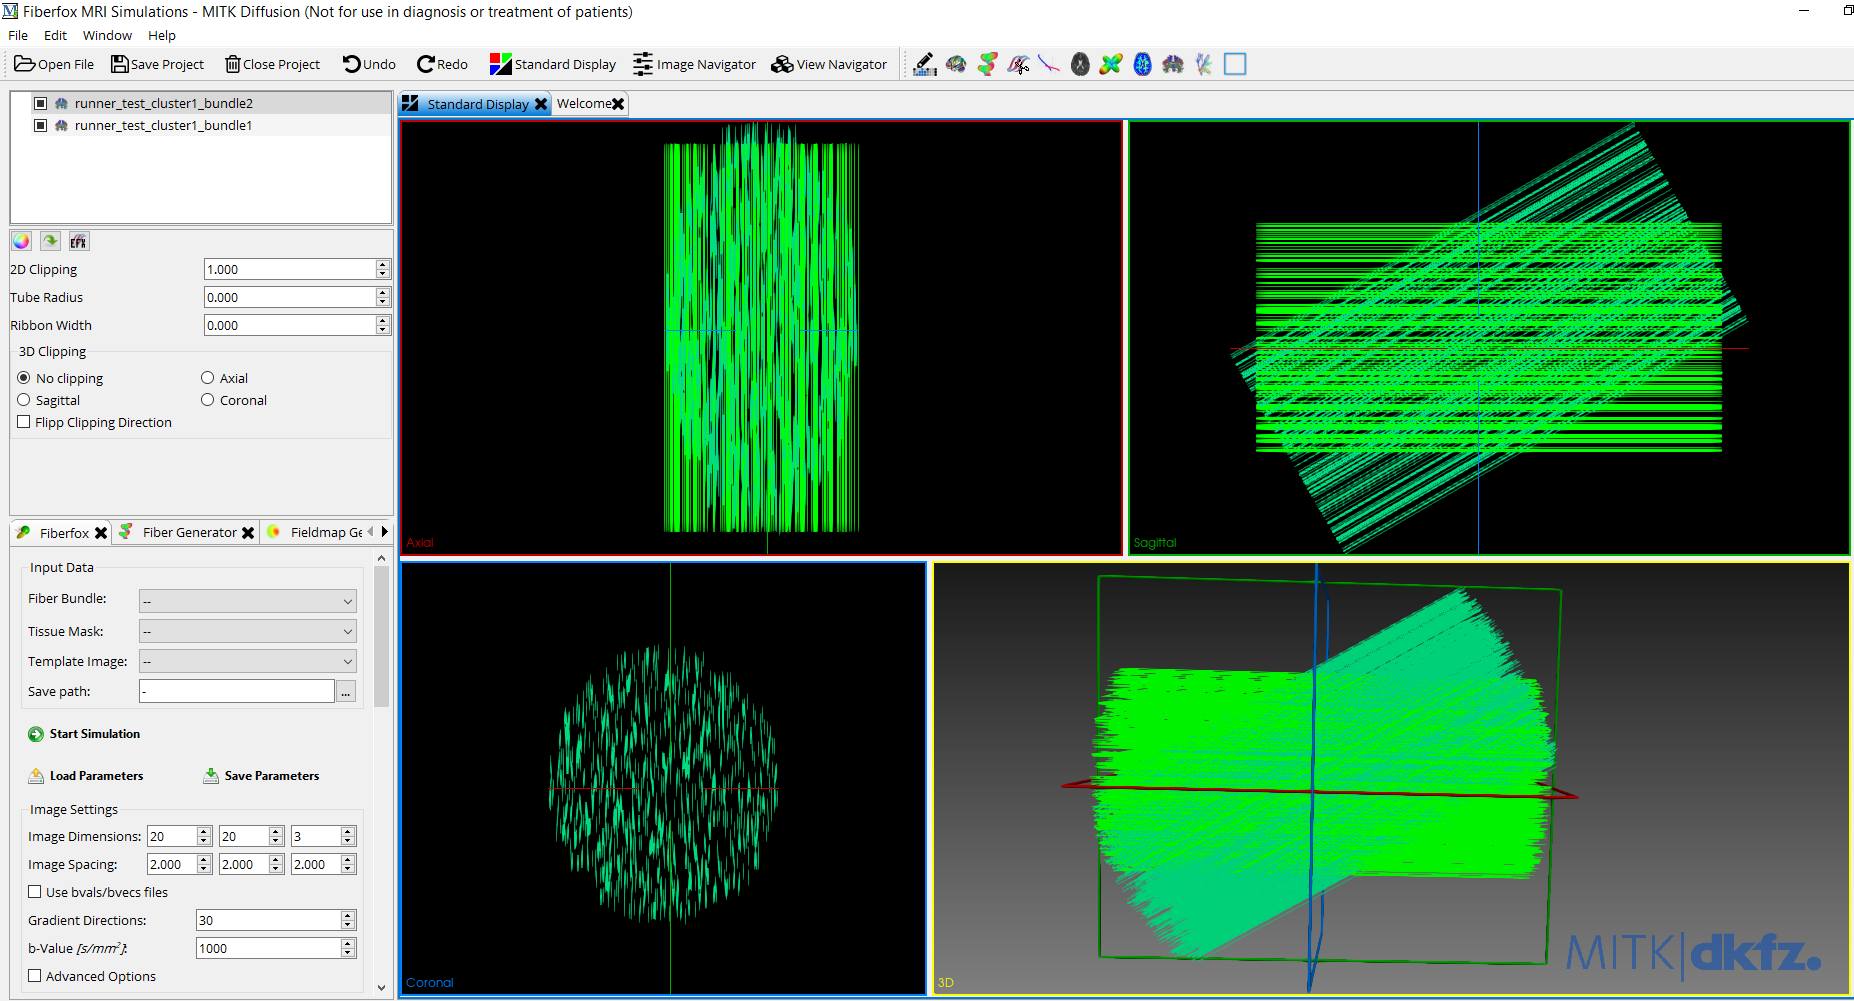
\includegraphics[width=\textwidth]{simulation_generator_results}
    \caption{Extrants de \textit{Simulation Generator} visualisés dans \textit{Fiberfox}}
    \label{fig:fig1}
  \end{figure}


  \section{Conclusion}
  \label{sec:conclusion}
  Parmi les logiciels scientifiques identifiés, seulement \textit{Simulation Generator} satisfait les exigences du projet.
  Celui-ci nous permet de générer des amas de fibres de matière blanche selon une configuration précise et flexible.
  De plus, les extrants du logiciel peuvent être visualisés aisément dans Fiberfox.
  En outre, son utilisation est automatisable, ergonomique et raisonnablement fonctionnellement indépendante.
  Aussi, \textit{Simulation Generator} a une interface de programmation en Python.

  Pour conclure, nous pourrons donc enchaîner avec le développement d'une application capable de générer des configurations précises d'amas de fibres de matière
  blanche, dans le but de valider nos nouveaux algorithmes de traitement de données de la microscopie par nappe de lumière (Light-sheet microscopy).


  \section*{Remerciements}
  \label{sec:thanks}
  Je souhaite remercier mon professeur-superviseur de recherche Joël Lefebvre qui m'a pris sous son aile et qui m'a formé sur les domaines du traitement d'images et
  de la neuroimagerie.


  % Ajoutez vos références (format bibtex) dans le fichier references.bib
  \bibliographystyle{unsrt}
  \bibliography{references}

\end{document}
